% arara: xelatex
% arara: xelatex
% arara: makeindex
% arara: xelatex until !found('log', 'Rerun to get ')
% arara: clean: { extensions: [ aux, idx, out, toc, ilg, ind ] }

\documentclass[11pt,a4paper]{ltxdoc}
\usepackage[margin=2cm]{geometry}

\usepackage[libertine]{newtxmath}
\usepackage[oldstyle]{libertine}
\usepackage{fontspec}
\setmonofont[Scale=0.8]{MesloLGS}[
  Path=fonts/,
  Extension=.ttf,
  UprightFont=*-Regular,
  BoldFont=*-Bold,
  ItalicFont=*-Italic,
  BoldItalicFont=*-BoldItalic
]

\usepackage{imakeidx}
\usepackage{tikzmusic}
\usepackage{pdfpages}

\setlength\parindent{0pt}

\def\pkg#1{{\sffamily #1}}
\def\tmname{\pkg{tikzmusic}}
\def\tikzname{Ti\emph{k}Z}
\def\pgfname{\textsc{pgf}}

% necessary for the manual styles:
\usepackage{calc}

% for cross-references:
\usepackage[unicode,pdftitle={The tikzmusic package},pdfauthor={Vu Van Dung},pdfborder=0 0 0]{hyperref}

\def\pgfautoxrefs{1}
\input{tikzmusic.macros.tex}

\makeatletter
\def\index@prologue{\section*{Index}\addcontentsline{toc}{section}{Index}}
\makeatother

% Automatic cross-referencing
\RequirePackage{pgfmanual}

% this here configures automatic cross referencing.
% It works for ANY package that uses pgfkeys and is independent on tikz/pgf. 
\pgfkeys{
  /pdflinks/search key prefixes in={/tm/},
  /pdflinks/internal link prefix=pgfp,
  /pdflinks/codeexample links=true,
  /pdflinks/warnings=false,   % for debugging 
  /pdflinks/show labels=false,% for debugging
}

% Resize it a bit
\let\oldtmline\tmline%
\def\tmline{\begin{minipage}{\linewidth-5mm}\oldtmline}%
\let\oldendtmline\endtmline%
\def\endtmline{\oldendtmline\end{minipage}}%

\makeindex

\title{The experimental \tmname\ package}
\author{Vũ Văn Dũng}
\date{Manual for version \tmversion\\Last compiled \today}

\begin{document}
\maketitle
\tableofcontents
\setlength\parskip{1ex}
\section{Introduction}\label{sec:intro}
\subsection{What it can do}\label{sec:intro:intro}
This package provides commands and syntaxes to help you draw musical notations in 
a \LaTeX\ document, based on the \tikzname\ package.

Note that this package is still \emph{very} experimental.
\subsection{Current limitations}\label{sec:intro:limitations}
Although the syntaxes are quite human-readable, they are very \emph{long}. In 
the future an easy-to-use front-end is necessary and should be implemented.

The speed is also an issue, as it requires time to draw many complex notations. 
For instance, the treble clef, |tm-g-clef|, takes $0.03$ seconds (in my machine) 
alone.\footnote{Thanks to the \pkg{l3benchmark} package.} This has no easy fix 
though, as efficiency and beauty, in these cases, can't live under the same roof.

There are many notations which are so advanced that I can't be confident enough 
to add them to the package. If you need them, feel free to submit a feature 
request to the \href{https://github.com/joulev/tikzmusic}{package repository}. 

Also, this documentation is written somewhat hastily, and may contain grammar 
mistakes from a non-native speaker. If you find typos or errors in the manual, 
feel free to send me a bug report.
\subsection{Thanks}\label{sec:intro:thanks}
First of all, I would like to thank the following people who have greatly 
helped me in writing this package:

\begin{itemize}
  % JouleV: I know this is an odd way to color hyperref, but anyway...
  \let\oldhref\href
  \def\href#1#2{\declare{\oldhref{#1}{#2}}}
  \item Till Tantau and every developer of the \tikzname-\pgfname\ package. 
  Obviously, without the powerful \pgfname\ and its easy-to-use front-end 
  \tikzname, this package, along with many others, would not be possible.
  \item The development team of all packages used by this package.
  \item Every member of the 
  \href{https://chat.stackoverflow.com/rooms/193903/duck-overflow}{Duck Overflow} 
  chat room and the \href{https://topanswers.xyz/tex}{Top\TeX} community, most 
  notably (but not limited to) marmot, samcarter and Skillmon, for their great 
  help in writing this package. My knowledge in \TeX\ and friends would not be 
  the same without these people.
  \item Christian Feuers\"anger for the |pgfmanual| documentation style, most 
  notably the automatic hyperlink in the documentation. The style was adopted 
  in the documentation of this package.
  \item The \href{https://inkscape.org/}{Inkscape} project and the 
  \href{https://github.com/kjellmf/svg2tikz}{\pkg{svg2tikz}} project. I have used these 
  two tools heavily to generate code for the musical notations from existing 
  SVG files. Although the files in {\sffamily tex/latex/tikzmusic/src/tm-paths} are 
  not automatically generated, most parts of them are generated by these tools.
  \item The \href{https://musescore.org}{MuseScore} project. Although I had known 
  some about music notations, that was too little for the package. I have used 
  MuseScore heavily for some ideas about music writing and music notations.
\end{itemize}

\section{Initialization}\label{sec:init}
\subsection{Loading the package}\label{sec:init:load}
This package currently only supports \LaTeXe.

\begin{package}{tikzmusic}
  Loading the \tmname\ package. There are no package options.
\end{package}

This package will automatically load the packages \pkg{spath3} 
and \tikzname, as well as \tikzname\ standard libraries |calc|, 
|intersection|, |decorations.pathreplacing|. You don't need to load these 
packages and libraries again in your document.
\subsection{Processing options}\label{sec:init:options}
The \tmname\ package uses the \pkg{pgfkeys} package to handle options. Every 
option defined in the package is in the same family, |/tm|, e.g. 
|color|.

\begin{command}{\tmset\marg{options}}
  Process \meta{options}. where the default path is set to |/tm|.
\end{command}

If you know about \tikzname\ and its key system, you can think |\tmset| 
works just like |\tikzset|, only the default path is different. You can now skip 
to the next section.

If you are not familiar with \pkg{pgfkeys} or |\pgfkeys| or 
|\tikzset|, \meta{options} is a list of \meta{key}\opt{|=|\meta{value}} 
pairs, separated by commas. The command will then separate each pair and process 
them.

\begin{itemize}
  \item If the key is with \meta{value}, option \meta{key}
  is processed, with its value being \meta{value}.
  \item Otherwise, the command will check whether \meta{key} is a defined key. 
  If it is defined, option \meta{key} is processed.
  \item Otherwise, the package will see if the \meta{key} is a valid color. If 
  so, it will be processed as the value for both |line color| and |color| 
  (see section \ref{sec:custom:color}).
  \item If it is not a valid color, the package will return an error.
\end{itemize}

If you want to learn deeper about this, you can read section 88 of the PGF 
manual (you can read it via |texdoc pgf|).
\subsection{Environments for music lines}\label{sec:init:drawing-environment}
Each music line will be drawn separately, by using the following environment:

\begin{environment}{{tmline}\opt{\oarg{options}}}
  Add a music line (consisting of one or many staves).
\end{environment}

\begin{codeexample}[]
\begin{tmline}[blue]
\begin{tmstaff}{g}{}\end{tmstaff}
\end{tmline}
\end{codeexample}

If a line consists of more than one staff, you may need to indent the staves a 
little bit to make room for instrument names and braces/brackets. You can do so 
by using the following key:

\begin{key}{/tm/staff offset=\meta{length} (initially 0pt)}
  Indent all staves in a line by \meta{length}.
\end{key}

\begin{codeexample}[]
\begin{tmline}[staff offset=1.5cm]
\begin{tmstaff}{g}{a}
  \path[overlay] (a-start) node[left] {Violin};%
\end{tmstaff}
\end{tmline}%
\end{codeexample}
\subsection{Creating a staff}\label{sec:init:staff-creation}
A staff can be created using one of the following environments:
\begin{environment}{{tmstaff}\opt{\oarg{options}}\marg{clef name}\marg{staff name}}
  Create a staff, with the starting clef is \meta{clef name}.

  \meta{clef name} can have three values: |g|, |f| and |c|, which stands for 
  the treble (G) clef, the bass (F) clef and the alto (C) clef, respectively.

  \meta{staff name} will be used to make cross-staff barlines or braces, so 
  you should only left it empty if you are sure you will not refer to it later.

  \meta{options} will be executed at the beginning of the environment.
\end{environment}
\begin{codeexample}[]
\begin{tmline}[staff offset=1cm]
\begin{tmstaff}{g}{}\end{tmstaff}
\end{tmline}
\end{codeexample}
\begin{environment}{{tmstaff*}\opt{\oarg{options}}\marg{staff name}}
  Work like |{tmstaff}|, but no clefs will be drawn.
\end{environment}
Essentially, |{tmstaff}| and |{tmstaff*}| are extensions of the 
|{tikzpicture}| environment, where the origin of the canva is the leftmost 
point of the middle line. That origin is marked as \tikzname\ remembered 
coordinate |(|\meta{staff name}|-start)|. There are also two other remembered 
coordinates: the leftmost points of the top line and the bottom line are marked 
as \tikzname\ coordinates |(|\meta{staff name}|-nw)| and |(|\meta{staff name}|-sw)| 
respectively.
\begin{codeexample}[]
\begin{tmline}
\begin{tmstaff}{g}{my-staff}
  \path (my-staff-nw) node[above,overlay] {1} ++ (.5,.5) node[right] {\bfseries Allegro};
\end{tmstaff}
\end{tmline}
\end{codeexample}
By default, the staff lines will be separated by |2mm|. You can scale this to 
a different value by using |scale|, see more in section \ref{sec:custom:transformations:scale}.

The lines will always span over the full line width, so to get a staff having 
some particular length, you can put them inside a |{minipage}|:
\def\tmline{\begin{minipage}{\linewidth}\oldtmline}%
\def\endtmline{\oldendtmline\end{minipage}}%
\begin{codeexample}[]
\begin{minipage}{4cm}
\begin{tmline}
\begin{tmstaff}{g}{}\end{tmstaff}
\end{tmline}
\end{minipage}
\end{codeexample}
\def\tmline{\begin{minipage}{\linewidth-5mm}\oldtmline}%
\def\endtmline{\oldendtmline\end{minipage}}%

\section{Multiple-staff operations}\label{sec:multistaff}
Because the following commands are multiple-staff commands, they should be 
used outside |{tmstaff}| and |{tmstaff*}| (\emph{except} 
|\tmbarlineinline|, |\tmdoublebarlineinline|, \dots).
\subsection{Ensembling staves}\label{sec:multistaff:ensemble-staves}
Braces that groups some staves inside a |{tmline}| can be drawn 
using the following command:
\begin{command}{\tmbrace\opt{\oarg{options}}\marg{staff 1}\marg{staff 2}\marg{text}}
  Draw a brace spanning from \meta{staff 1} to \meta{staff 2}. 
  \meta{text} is displayed at the middle of the brace. If you don't want 
  any text to be displayed, you can leave this option empty.
\end{command}
% Vu Van Dung: Inside the {codeexample} environment, indenting 
% everything outside {tmstaff} or {tmstaff*} causes a blank 
% line to be inserted, which is not the case for any other 
% cases. I don't know why.
\begin{codeexample}[]
\begin{tmline}[staff offset=2cm]%
\begin{tmstaff}{g}{piano-1}\end{tmstaff}%
\begin{tmstaff}{f}{piano-2}\end{tmstaff}%
\tmbrace{piano-1}{piano-2}{Piano}%
\end{tmline}
\end{codeexample}
Similarly, brackets can also be drawn:
\begin{command}{\tmbracket\opt{\oarg{options}}\marg{staff 1}\marg{staff 2}}
  Draw a bracket spanning from \meta{staff 1} to \meta{staff 2}. 
  Unlike |\tmbrace|, no text will be displayed.
\end{command}
\begin{codeexample}[]
\begin{tmline}[staff offset=2.5cm]%
\begin{tmstaff}{g}{Violin}\end{tmstaff}%
\begin{tmstaff}{c}{Viola}\end{tmstaff}%
\begin{tmstaff}{f}{Violoncello}\end{tmstaff}%
\begin{tikzpicture}[remember picture,overlay]
  \foreach \i in {Violin,Viola,Violoncello}\path (\i-start) node[left=2mm] {\i};
\end{tikzpicture}%
\tmbracket{Violin}{Violoncello}%
\end{tmline}
\end{codeexample}
\subsection{Barlines}\label{sec:multistaff:barlines}
The \tmname\ package supports many different types of barlines. 
\subsubsection{Normal barlines}\label{sec:multistaff:barlines:normal}
\begin{command}{\tmbarline\opt{\oarg{options}}\marg{x-pos}\marg{staff}}
  Draw a normal barline on \meta{staff} at $x$-position \meta{x-pos} in 
  relative to the origin |(|\meta{staff}|-start)|. 
\end{command}
\begin{codeexample}[]
\begin{tmline}%
\begin{tmstaff}{g}{staff-1}\end{tmstaff}%
\begin{tmstaff}{f}{staff-2}\end{tmstaff}%
\tmbarline{5}{staff-1}%
\tmbarline[teal]{5}{staff-2}%
\end{tmline}
\end{codeexample}
% JouleV: No, starred commands don't work :(
\begin{command}{\tmbarline*\opt{\oarg{options}}\marg{x-pos}\marg{staff 1}\marg{staff 2}}
  Draw a normal barline spanning from \meta{staff 1} to 
  \meta{staff 2}, at $x$-position \meta{x-pos} in relative to 
  the origin |(|\meta{staff name}|-start)| of either staff.
\end{command}
\begin{codeexample}[]
\begin{tmline}%
\begin{tmstaff}{g}{staff-1}\end{tmstaff}%
\begin{tmstaff}{f}{staff-2}\end{tmstaff}%
\tmbarline*{5}{staff-1}{staff-2}%
\end{tmline}
\end{codeexample}
A special case of |\tmbarline*| is implemented in the following command:
\begin{command}{\tmbarlineendline\opt{\oarg{options}}\marg{staff 1}\marg{staff 2}}
  Draw a normal barline spanning from \meta{staff 1} to 
  \meta{staff 2} at the end of the line.
\end{command}
\begin{codeexample}[]
\begin{tmline}
\begin{tmstaff}{g}{staff-1}\end{tmstaff}%
\begin{tmstaff}{c}{staff-2}\end{tmstaff}%
\begin{tmstaff}{f}{staff-3}\end{tmstaff}%
\tmbarline*{0}{staff-1}{staff-3}%
\tmbarlineendline[blue]{staff-1}{staff-3}%
\end{tmline}
\end{codeexample}
If you want to draw the barline inside |{tmstaff}| or |{tmstaff*}|, 
you can use 
\begin{command}{\tmbarlineinline\opt{\oarg{options}}\marg{list of x-pos}}
  Draw a normal barline at each $x$-position specified in \marg{list of x-pos}.
\end{command}
\begin{codeexample}[]
\begin{tmline}%
\begin{tmstaff}{g}{}
  \tmbarlineinline[blue]{3,5,8,9}
\end{tmstaff}%
\end{tmline}
\end{codeexample}
\subsubsection{Double barlines}\label{sec:multistaff:barlines:double}
Like when drawing normal barlines as described in section 
\ref{sec:multistaff:barlines:normal}, 
we also have four commands for double barlines.
\begin{command}{\tmdoublebarline\opt{\oarg{options}}\marg{x-pos}\marg{staff}}
  Draw a double barline on \meta{staff} at $x$-position \meta{x-pos} in 
  relative to the origin |(|\meta{staff}|-start)|.
\end{command}
\begin{command}{\tmdoublebarline*\opt{\oarg{options}}\marg{x-pos}\marg{staff 1}\marg{staff 2}}
  Draw a double barline spanning from \meta{staff 1} to 
  \meta{staff 2}, at $x$-position \meta{x-pos} in relative to 
  the origin |(|\meta{staff name}|-start)| of either staff.
\end{command}
\begin{command}{\tmdoublebarlineendline\opt{\oarg{options}}\marg{staff 1}\marg{staff 2}}
  Draw a double barline spanning from \meta{staff 1} to 
  \meta{staff 2} at the end of the line.
\end{command}
\begin{command}{\tmdoublebarlineinline\opt{\oarg{options}}\marg{list of x-pos}}
  Draw a double barline at each $x$-position specified in \marg{list of x-pos}.
\end{command}
Example use of all four commands described in this section:
\begin{codeexample}[]
\begin{tmline}%
\begin{tmstaff}{g}{staff-1}\end{tmstaff}%
\begin{tmstaff}{f}{staff-2}
  \tmdoublebarlineinline{8,9,10}
\end{tmstaff}%
\tmbarline*{0}{staff-1}{staff-2}%
\tmdoublebarline*{4}{staff-1}{staff-2}%
\tmdoublebarline{7}{staff-1}%
\tmdoublebarlineendline{staff-1}{staff-2}%
\end{tmline}
\end{codeexample}
\subsubsection{Dotted barlines}\label{sec:multistaff:barlines:dotted}
Now you can see the patterns :).
\begin{command}{\tmdottedbarline\opt{\oarg{options}}\marg{x-pos}\marg{staff}}
  Draw a dotted barline on \meta{staff} at $x$-position \meta{x-pos} in 
  relative to the origin |(|\meta{staff}|-start)|.
\end{command}
\begin{command}{\tmdottedbarline*\opt{\oarg{options}}\marg{x-pos}\marg{staff 1}\marg{staff 2}}
  Draw a dotted barline spanning from \meta{staff 1} to 
  \meta{staff 2}, at $x$-position \meta{x-pos} in relative to 
  the origin |(|\meta{staff name}|-start)| of either staff.
\end{command}
\begin{command}{\tmdottedbarlineendline\opt{\oarg{options}}\marg{staff 1}\marg{staff 2}}
  Draw a dotted barline spanning from \meta{staff 1} to 
  \meta{staff 2} at the end of the line.
\end{command}
\begin{command}{\tmdottedbarlineinline\opt{\oarg{options}}\marg{list of x-pos}}
  Draw a double barline at each $x$-position specified in \marg{list of x-pos}.
\end{command}
The commands in use:
\begin{codeexample}[]
\begin{tmline}%
\begin{tmstaff}{g}{staff-1}\end{tmstaff}%
\begin{tmstaff}{f}{staff-2}
  \tmdottedbarlineinline{8,9,10}
\end{tmstaff}%
\tmbarline*{0}{staff-1}{staff-2}%
\tmdottedbarline*{4}{staff-1}{staff-2}%
\tmdottedbarline{7}{staff-1}%
\tmdottedbarlineendline{staff-1}{staff-2}%
\end{tmline}
\end{codeexample}
\subsubsection{Final barlines}\label{sec:multistaff:barlines:final}
\begin{command}{\tmfinalbarline\opt{\oarg{options}}\marg{x-pos}\marg{staff}}
  Draw a final barline on \meta{staff} at $x$-position \meta{x-pos} in 
  relative to the origin |(|\meta{staff}|-start)|.
\end{command}
\begin{command}{\tmfinalbarline*\opt{\oarg{options}}\marg{x-pos}\marg{staff 1}\marg{staff 2}}
  Draw a final barline spanning from \meta{staff 1} to 
  \meta{staff 2}, at $x$-position \meta{x-pos} in relative to 
  the origin |(|\meta{staff name}|-start)| of either staff.
\end{command}
\begin{command}{\tmfinalbarlineendline\opt{\oarg{options}}\marg{staff 1}\marg{staff 2}}
  Draw a final barline spanning from \meta{staff 1} to 
  \meta{staff 2} at the end of the line.
\end{command}
\begin{command}{\tmfinalbarlineinline\opt{\oarg{options}}\marg{list of x-pos}}
  Draw a final barline at each $x$-position specified in \marg{list of x-pos}.
\end{command}
\begin{codeexample}[]
\begin{tmline}%
\begin{tmstaff}{g}{staff-1}\end{tmstaff}%
\begin{tmstaff}{f}{staff-2}
  \tmfinalbarlineinline{8,9,10}
\end{tmstaff}%
\tmbarline*{0}{staff-1}{staff-2}%
\tmfinalbarline*{4}{staff-1}{staff-2}%
\tmfinalbarline{7}{staff-1}%
\tmfinalbarlineendline{staff-1}{staff-2}%
\end{tmline}
\end{codeexample}
\subsubsection{Start repeat barlines}\label{sec:multistaff:barlines:start}
\begin{command}{\tmstartrepeatbarline\opt{\oarg{options}}\marg{x-pos}\marg{staff}}
  Draw a start repeat barline on \meta{staff} at $x$-position \meta{x-pos} in 
  relative to the origin |(|\meta{staff}|-start)|.
\end{command}
\begin{command}{\tmstartrepeatbarline*\opt{\oarg{options}}\marg{x-pos}\marg{staff 1}\marg{staff 2}\marg{list of staff names}}
  Draw a start repeat barline spanning from \meta{staff 1} to 
  \meta{staff 2}, at $x$-position \meta{x-pos} in relative to 
  the origin |(|\meta{staff name}|-start)| of either staff.

  Because of some internal problems, you need to specify a full list of the names 
  of the staff that the barline spans over in \meta{list of staff names} with 
  a comma-separated list.
\end{command}
\begin{command}{\tmstartrepeatbarlineinline\opt{\oarg{options}}\marg{list of x-pos}}
  Draw a start repeat barline at each $x$-position specified in \marg{list of x-pos}.
\end{command}
\begin{codeexample}[]
\begin{tmline}%
\begin{tmstaff}{g}{staff-1}\end{tmstaff}%
\begin{tmstaff}{f}{staff-2}
  \tmstartrepeatbarlineinline{8,9,10}
\end{tmstaff}%
\tmbarline*{0}{staff-1}{staff-2}%
\tmstartrepeatbarline*{4}{staff-1}{staff-2}{staff-1,staff-2}%
\tmstartrepeatbarline{7}{staff-1}%
\end{tmline}
\end{codeexample}
Note that there is no |\tmstartrepeatbarlineendline|, because I am sure you 
will never put a start repeat barline to the end of a line.
\subsubsection{End repeat barlines}\label{sec:multistaff:barlines:end}
\begin{command}{\tmendrepeatbarline\opt{\oarg{options}}\marg{x-pos}\marg{staff}}
  Draw an end repeat barline on \meta{staff} at $x$-position \meta{x-pos} in 
  relative to the origin |(|\meta{staff}|-start)|.
\end{command}
\begin{command}{\tmendrepeatbarline*\opt{\oarg{options}}\marg{x-pos}\marg{staff 1}\marg{staff 2}\marg{list of staff names}}
  Draw an end repeat barline spanning from \meta{staff 1} to 
  \meta{staff 2}, at $x$-position \meta{x-pos} in relative to 
  the origin |(|\meta{staff name}|-start)| of either staff.

  Similar to |\tmstartrepeatbarline*|, you also need to specify 
  \meta{list of staff names.}
\end{command}
\begin{command}{\tmendrepeatbarlineendline\opt{\oarg{options}}\marg{staff 1}\marg{staff 2}\marg{list of staff names}}
  Draw an end repeat barline spanning from \meta{staff 1} to 
  \meta{staff 2} at the end of the line. 
\end{command}
\begin{command}{\tmendrepeatbarlineinline\opt{\oarg{options}}\marg{list of x-pos}}
  Draw a end repeat barline at each $x$-position specified in \marg{list of x-pos}.
\end{command}
\begin{codeexample}[]
\begin{tmline}%
\begin{tmstaff}{g}{staff-1}\end{tmstaff}%
\begin{tmstaff}{f}{staff-2}
  \tmendrepeatbarlineinline{8,9,10}
\end{tmstaff}%
\tmbarline*{0}{staff-1}{staff-2}%
\tmendrepeatbarline*{4}{staff-1}{staff-2}{staff-1,staff-2}%
\tmendrepeatbarline{7}{staff-1}%
\tmendrepeatbarlineendline{staff-1}{staff-2}{staff-1,staff-2}%
\end{tmline}
\end{codeexample}
\subsubsection{End-start repeat barlines}\label{sec:multistaff:barlines:endstart}
Sometimes, you want a barline to be a start repeat barline and an end repeat 
barline at the same time. You should not use |\tmstartrepeatbarline| (and 
similar commands) and |\tmendrepeatbarline| (and similar commands) at the 
same place, because it will look very bad. In those cases, use the following 
commands:
\begin{command}{\tmendstartrepeatbarline\opt{\oarg{options}}\marg{x-pos}\marg{staff}}
  Draw an `end-start' repeat barline on \meta{staff} at $x$-position 
  \meta{x-pos} in relative to the origin |(|\meta{staff}|-start)|.
\end{command}
\begin{command}{\tmendstartrepeatbarline*\opt{\oarg{options}}\marg{x-pos}\marg{staff 1}\marg{staff 2}\marg{list of staff names}}
  Draw an `end-start' repeat barline spanning from \meta{staff 1} to 
  \meta{staff 2}, at $x$-position \meta{x-pos} in relative to 
  the origin |(|\meta{staff name}|-start)| of either staff.
\end{command}
\begin{command}{\tmendstartrepeatbarlineinline\opt{\oarg{options}}\marg{list of x-pos}}
  Draw a end repeat barline at each $x$-position specified in \marg{list of x-pos}.
\end{command}
\begin{codeexample}[]
\begin{tmline}%
\begin{tmstaff}{g}{staff-1}\end{tmstaff}%
\begin{tmstaff}{f}{staff-2}
  \tmendstartrepeatbarlineinline{8,9,10}
\end{tmstaff}%
\tmbarline*{0}{staff-1}{staff-2}%
\tmendstartrepeatbarline*{4}{staff-1}{staff-2}{staff-1,staff-2}%
\tmendstartrepeatbarline{7}{staff-1}%
\end{tmline}
\end{codeexample}
Note that there is no |\tmendstartrepeatbarlineendline|.
\subsubsection{Normal barlines loops}\label{sec:multistaff:barlines:normal-loop}
Normally there are many barlines in your line, so using |\tmbarline| for 
each of them is obviously not convenient. You can use the following commands 
to make drawing barlines easier and more concise.
\begin{command}{\tmbarlineloop\opt{\oarg{options}}\marg{list of x-pos}\marg{list of staff names}}
  Draw a normal barline at each $x$-position in \meta{list of x-pos} and at each 
  staff specified in \meta{list of staff names}.
\end{command}
\begin{codeexample}[]
\begin{tmline}%
  \begin{tmstaff}{g}{staff-1}\end{tmstaff}%
  \begin{tmstaff}{f}{staff-2}\end{tmstaff}%
  \tmbarlineloop{3,6,9}{staff-1,staff-2}%
\end{tmline}
\end{codeexample}
\begin{command}{\tmbarlineloop*\opt{\oarg{options}}\marg{list of x-pos}\marg{staff 1}\marg{staff 2}}
  Draw a normal barline at each $x$-position in \meta{list of x-pos}, spanning 
  from \meta{staff 1} to \meta{staff 2}.
\end{command}
\begin{codeexample}[]
\begin{tmline}%
\begin{tmstaff}{g}{staff-1}\end{tmstaff}%
\begin{tmstaff}{f}{staff-2}\end{tmstaff}%
\tmbarlineloop*{3,6,9}{staff-1}{staff-2}%
\end{tmline}
\end{codeexample}

\section{Key signatures and time signatures}\label{sec:signatures}
\subsection{Key signatures}\label{sec:signatures:key}
Key signatures are added by the following command:
\begin{command}{\tmkeysignature\opt{\oarg{options}}\marg{x-pos}\marg{type}\marg{number}}
  Add a key signature at $x$-position \meta{x-pos}. The key signature has type 
  \meta{type} and the number of \mbox{sharps/flats} \meta{number}.

  \meta{type} can be either |sharp|, |flat|, |nsharp| or |nflat|. |sharp| and 
  |flat| will produce a sharp or flat key signature as usual. |nsharp| and 
  |nflat| will produce a `natural' key signature that has the format of sharp and 
  flat, respectively.
  
  \meta{number} can be any number from |1| to |7|.

  The key signature will be added as in a treble clef. You can use shifting options, 
  e.g. |line shift| (see more in section \ref{sec:custom:transformations}) 
  to shift the key signature so that it fits other clefs.
\end{command}
\begin{codeexample}[]
\begin{tmline}
\begin{tmstaff}{g}{}
  \tmkeysignature{3}{sharp}{5}
  \tmkeysignature{5}{nsharp}{5}
  \tmkeysignature{7}{flat}{5}
  \tmkeysignature{9}{nflat}{5}
\end{tmstaff}
\end{tmline}
\end{codeexample}
\subsection{Time signatures}\label{sec:signatures:time}
Normal time signatures can be added using the following command
\begin{command}{\tmtimesignature\opt{\oarg{options}}\marg{x-pos}\marg{upper}\marg{lower}}
  Add a time signature to $x$-position \meta{x-pos}. The upper part and the lower 
  part of the time signature are \meta{upper} and \meta{lower} respectively.
\end{command}
\begin{codeexample}[]
\begin{tmline}[staff offset=2cm]%
\begin{tmstaff}{g}{piano-1}
  \tmkeysignature{1}{sharp}{5}\tmtimesignature{2.5}{12}{8}
\end{tmstaff}%
\begin{tmstaff}{f}{piano-2}
  \tmkeysignature[line shift=-2]{1}{sharp}{5}\tmtimesignature{2.5}{12}{8}
\end{tmstaff}%
\tmbrace{piano-1}{piano-2}{Piano}%
\tmbarline{0}{piano-1}{piano-2}\tmbarlineendline{piano-1}{piano-2}%
\end{tmline}
\end{codeexample}
Special time signatures have their own commands:
\begin{command}{\tmtimesignaturecommon\opt{\oarg{options}}\marg{x-pos}}
  Add the common time signature (\tikz\pic{tm-common-time};) to $x$-position 
  \meta{x-pos}.
\end{command}
\begin{command}{\tmtimesignatureallabreve\opt{\oarg{options}}\marg{x-pos}}
  Add the alla breve time signature (\tikz\pic{tm-alla-breve-time};) to $x$-position 
  \meta{x-pos}.
\end{command}
\begin{codeexample}[]
\begin{tmline}%
\begin{tmstaff}{g}{helloworld}
  \tmkeysignature{1}{flat}{3}
  \tmtimesignaturecommon{2}
  \tmtimesignatureallabreve[yshift=3mm]{6.5}
\end{tmstaff}%
\tmbarline{6}{helloworld}{helloworld}\tmfinalbarlineendline{helloworld}{helloworld}%
\end{tmline}
\end{codeexample}

\section{Adding notes}\label{sec:music-notes}
\subsection{Commands for notes}\label{sec:music-notes:commands}
\subsubsection{Note values}\label{sec:music-notes:commands:note-values}
\begin{figure}[t]
  \centering
  \caption{Note value -- the letter part}
  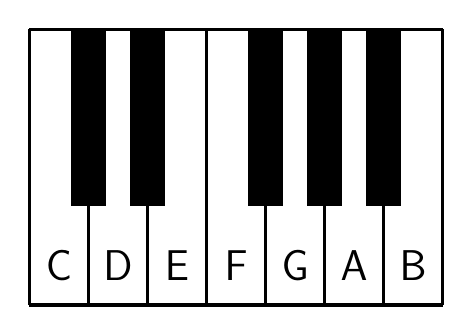
\begin{tikzpicture}[y=1cm/1.5,scale=0.75,transform shape]
    \draw[very thick,fill=white] (0,0) grid[xstep=1,ystep=7] (7,7);
    \foreach \i in {1,2,4,5,6}
      \fill (\i-.3,2.5) rectangle (\i+.3,7);
    \foreach \i [count=\j] in {C,D,E,F,G,A,B}
      \path (\j-.5,1) node[font=\huge\sffamily] {\i};
  \end{tikzpicture}
  \label{fig:music-notes:commands:note-values:letter}
\end{figure}
\begin{figure}[t]
  \centering
  \caption{Note value -- the number part}
  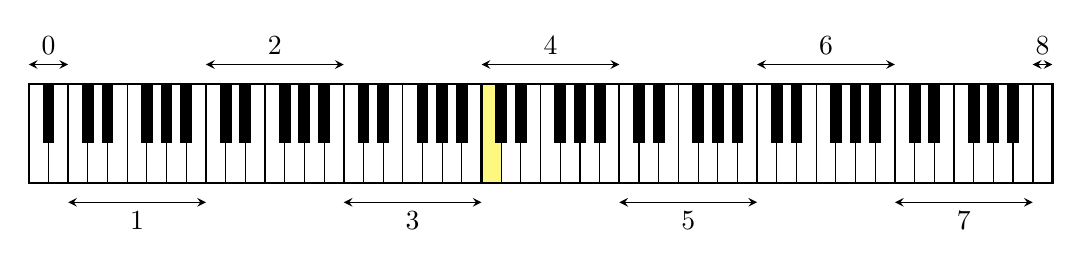
\begin{tikzpicture}[x=0.25cm,y=0.25cm,>=stealth]
    \fill[yellow!50] (23,0) rectangle (24,5);
    \draw (0,0) grid[xstep=1,ystep=5] (52,5);
    \draw[thick,shift={(2,0)}] (0,0) grid[xstep=7,ystep=5] (49,5);
    \draw[thick] (0,0) rectangle (2,5) (51,5) rectangle (52,0);
    \foreach \i in {1,...,7} {
      \foreach \j in {1,2,4,5,6} {
        \fill[shift={({2+(\i-1)*7},0)}] (\j-.3,2) rectangle (\j+.3,5);
      }
    }
    \fill (.7,2) rectangle (1.3,5);
    \foreach \i in {1,...,7} {
      \ifodd\i
        \draw[<->] ({(\i-1)*7+2},-1) -- ++ (7,0) node[midway,below] {\i};
      \else
        \draw[<->] ({(\i-1)*7+2},6) -- ++ (7,0) node[midway,above] {\i};
      \fi
    }
    \draw[<->] (0,6) -- (2,6) node[midway,above] {0};
    \draw[<->] (51,6) -- (52,6) node[midway,above] {8};
  \end{tikzpicture}
  \label{fig:music-notes:commands:note-values:number}
\end{figure}
Every white note is assigned to a `value', which is the \emph{scientific pitch 
notation} of that note. These values have two parts: the letter part and the 
number part:
\begin{itemize}
  \item The letter part can have seven values: |A|, |B|, |C|, \dots, |G|, 
  indicating the name of the note (\emph{do}, \emph{re}, \emph{mi}, \dots). (See 
  figure \ref{fig:music-notes:commands:note-values:letter}).
  \item The number part is a whole number between $0$ to $8$, indicating which 
  octave the note is in. (See figure \ref{fig:music-notes:commands:note-values:number}).
\end{itemize}
For example, \emph{F\"ur Elise} by Beethoven starts with an |E5| (a \emph{mi} at the 
5th octave).

We will only work with these values. To have black notes in your score, you can 
use |accidental| to add the accidentals, see more in section \ref{sec:music-notes:misc:accidentals}.

The package will automatically detect which staff you are using, when you use 
these values.
\subsubsection{Note names}\label{sec:music-notes:commands:note-names}
It is very possible that a note will be refered to later in the staff (to add 
notations to it, etc.). In this package, to refer to notes, we will use note 
\emph{names}. Just like \tikzname\ node names, etc. -- you can leave the name 
empty if you want, but you will not be able to communicate with that unnamed note 
any time later in the document.
\subsubsection{Whole notes}\label{sec:music-notes:commands:whole}
\begin{command}{\tmwhole\opt{\oarg{options}}\marg{x-pos}\marg{note value list}\marg{name}}
  Add a set of whole notes at $x$-position \meta{x-pos}. Each value in the 
  comma-separated list \meta{note value list} corresponds to a note. Note that 
  if you want to pass options to some notes, you can prefix \oarg{options} to the 
  beginning of the note name, e.g. |\tmwhole{4}{[red]C4,E4}{a}|.

  \meta{name} can be left empty, but as in the staff naming, I strongly advise 
  you to find some name for each note set.

  The center of note with note value $x$ will be marked as coordinate 
  |(|\meta{name}|-|$x$|)|. For example, note |F5| will be marked as 
  |(|\meta{name}|-F5)|. Also, the point on the middle line of the staff which is 
  at \meta{x-pos} will be marked as |(|\meta{name}|-center)|.
\end{command}
\begin{codeexample}[]
\begin{tmline}
\begin{tmstaff}{g}{}
  \tmwhole{3}{C4,E4,G4}{c-major}\tmwhole{5}{A4,C5,E5}{a-minor}
\end{tmstaff}
\end{tmline}
\end{codeexample}
\subsubsection{Relative positioning}\label{sec:music-notes:commands:relative}
Consider the following example:
\begin{codeexample}[]
\begin{tmline}
\begin{tmstaff}{g}{}
  \tmwhole{5}{D4,F4,G4}{}% G7
\end{tmstaff}
\end{tmline}
\end{codeexample}
It looks very bad, doesn't it? Note |G4| should be shifted a bit to the right. 
You can achieve this by using the following key:
\begin{key}{/tm/relative=\meta{relative position} (initially center)}
  Apply relative position to the note. \meta{relative position} can be either 
  |center|, |left| or |right|.
\end{key}
\begin{codeexample}[]
\begin{tmline}
\begin{tmstaff}{g}{}
  \tmwhole{5}{D4,[relative=right]F4,G4}{}
\end{tmstaff}
\end{tmline}
\end{codeexample}
\subsubsection{Half notes}\label{sec:music-notes:commands:half}
\begin{command}{\tmhalf\opt{\oarg{options}}\marg{x-pos}\marg{note value list}\marg{name}}
  Add a half note at position \meta{x-pos}. The stem direction will be automatically 
  determined.
\end{command}
The end of the stem is marked as coordinate |(|\meta{name}|-tail)|. (This also 
applies to |\tmquarter|, |\tmeighth| and |\tmmorethaneighth|.)
\begin{codeexample}[]
\begin{tmline}%
\begin{tmstaff}{g}{}
  \tmhalf{2}{E4}{}\tmhalf{3}{F5}{}\tmhalf{4}{E4,F5}{}\tmhalf{5}{B4}{}
  \tmhalf[reversed]{6}{E4}{}      \tmhalf[reversed]{7}{F5}{}
  \tmhalf[reversed]{8}{E4,F5}{}   \tmhalf[reversed]{9}{B4}{}
  \tmhalf{11}{[relative=left]F4,B4,G4,[relative=right]C5}{}
\end{tmstaff}%
\end{tmline}
\end{codeexample}
\subsubsection{Stem direction}\label{sec:music-notes:commands:stem-direction}
You can change the default direction of the stem by using |reversed|, see the 
following example and section \ref{sec:custom:reverse}.
\begin{codeexample}[]
\begin{tmline}
\begin{tmstaff}{g}{}
  \tmhalf{3}{C5}{}\tmhalf[reversed]{6}{C5}{}
\end{tmstaff}
\end{tmline}
\end{codeexample}
\subsubsection{Quarter notes}\label{sec:music-notes:commands:quarter}
\begin{command}{\tmquarter\opt{\oarg{options}}\marg{x-pos}\marg{note value list}\marg{name}}
  Similar to |\tmhalf|.
\end{command}
\begin{codeexample}[]
\begin{tmline}%
\begin{tmstaff}{g}{}
  \tmquarter{2}{E4}{}\tmquarter{3}{F5}{}\tmquarter{4}{E4,F5}{}\tmquarter{5}{B4}{}
  \tmquarter[reversed]{6}{E4}{}         \tmquarter[reversed]{7}{F5}{}
  \tmquarter[reversed]{8}{E4,F5}{}      \tmquarter[reversed]{9}{B4}{}
  \tmquarter{11}{[relative=left]F4,B4,G4,[relative=right]C5}{}
\end{tmstaff}%
\end{tmline}
\end{codeexample}
\subsubsection{Eighth notes}\label{sec:music-notes:commands:eighth}
\begin{command}{\tmeighth\opt{\oarg{options}}\marg{x-pos}\marg{note value list}\marg{name}}
  Similar to |\tmhalf|.
\end{command}
\begin{codeexample}[]
\begin{tmline}%
\begin{tmstaff}{g}{}
  \tmeighth {2}{E4}{}\tmeighth{3}{F5}{}\tmeighth{4}{E4,F5}{}\tmeighth{5}{B4}{}
  \tmeighth[reversed]{6}{E4}{}         \tmeighth[reversed]{7}{F5}{}
  \tmeighth[reversed]{8}{E4,F5}{}      \tmeighth[reversed]{9}{B4}{}
  \tmeighth{11}{[relative=left]F4,B4,G4,[relative=right]C5}{}
\end{tmstaff}%
\end{tmline}
\end{codeexample}
\subsubsection{More than eighth notes}\label{sec:music-notes:commands:more-than-eighth}
The commands described in this section applies to every notes below the eighth 
notes, including the sixteenth note (semiquaver), the thirty-second note 
(demisemiquaver), etc.
\begin{command}{\tmmorethaneighth\opt{\oarg{options}}\marg{x-pos}\marg{note value list}\marg{number of flags}\marg{name}}
  Similar to |\tmhalf|.
\end{command}
\begin{codeexample}[]
\begin{tmline}%
\begin{tmstaff}{g}{}
  \tmmorethaneighth{2}{F4}{2}{note-2}
  \tmmorethaneighth{3}{F4}{3}{note-3}
  \tmmorethaneighth{4}{F4}{4}{note-4}
  \tmmorethaneighth{5}{F4}{5}{note-5}
  \tmmorethaneighth{6}{F4}{6}{note-6}
\end{tmstaff}%
\end{tmline}
\end{codeexample}
\subsubsection{Grace notes}\label{sec:music-notes:commands:grace}
You can use |scale| to have smaller notes:
\begin{codeexample}[]
\begin{tmline}
\begin{tmstaff}{g}{}
  \tmeighth[scale=.6]{5}{A4}{a}\tmquarter[reversed]{5.5}{B4}{b}
  \tmslur[amplitude=1mm]{a}{b}
\end{tmstaff}
\end{tmline}
\end{codeexample}
To strike the note, you can use the following key:
\begin{key}{/tm/grace strike out=\meta{|true| or |false|} (default true)}
  Strike the grace note.
\end{key}
\begin{codeexample}[]
\begin{tmline}
\begin{tmstaff}{g}{}
  \tmeighth[scale=.6,grace strike out]{5}{A4}{}\tmeighth[grace strike out]{7}{A4}{}
\end{tmstaff}
\end{tmline}
\end{codeexample}
\subsection{Beaming}\label{sec:music-notes:beam}
\begin{environment}{{tmbeam}\opt{\oarg{options}}}
  Add a beaming note series. All notes inside this environment are `beamed' 
  together, and all stems point {\bfseries upwards}.
\end{environment}
\begin{environment}{{tmbeam*}\opt{\oarg{options}}}
  Identical to |{tmbeam}|, only all stems point {\bfseries downwards}.
\end{environment}
\emph{All} notes to be beamed inside these environments need to be added using 
the following command (|\tmeighth|, \dots\ will simply not work):
\begin{command}{\tmbeamnote\opt{\oarg{options}}\marg{x-pos}\marg{note value}\marg{number of flags}\marg{name}}
  Add a note to the beaming series. If \meta{number of flags} is $1$, it is an 
  eighth note, if \meta{number of flags} is $2$, it is a sixteenth note, and so 
  on.
\end{command}
{\bfseries\sffamily Important note:} Because of the algorithm working 
behind the scene, you \emph{must} give a separate name to each |\tmbeamnote| 
inside |{tmbeam}| or |{tmbeam*}|. Doing otherwise will result in 
weird output.
\begin{codeexample}[]
\begin{tmline}%
\begin{tmstaff}{g}{p1}
  \tmtimesignature{1}{3}{8}
  \begin{tmbeam*}
    \tmbeamnote{1.75}{E5}{2}{}\tmbeamnote{2.5}{[accidental=sharp]D5}{2}{a}
  \end{tmbeam*}
  \tmbarlineinline{2.8}
  \begin{tmbeam*}
    \tmbeamnote{3.25}{E5}{2}{a}\tmbeamnote{4}{[accidental=sharp]D5}{2}{b}\tmbeamnote{4.5}{E5}{2}{c}
    \tmbeamnote{5}{B4}{2}{d}\tmbeamnote{5.5}{[accidental=natural]D5}{2}{e}\tmbeamnote{6}{C5}{2}{f}
  \end{tmbeam*}
  \tmbarlineinline{6.3}\tmeighth[dot=1]{6.75}{A4}{a}
  \begin{tmbeam}
    \tmbeamnote{8}{C4}{2}{a}\tmbeamnote{8.5}{E4}{2}{b}\tmbeamnote{9}{A4}{2}{c}
  \end{tmbeam}
  \tmbarlineinline{9.3}\tmeighth[dot=1]{9.75}{B4}{a}
  \begin{tmbeam}
    \tmbeamnote{10.75}{E4}{2}{a}\tmbeamnote{11.5}{[accidental=sharp]G4}{2}{b}\tmbeamnote{12}{B4}{2}{c}
  \end{tmbeam}
  \tmbarlineinline{12.3}\tmquarter[dot=1]{12.75}{C5}{a}
\end{tmstaff}%
\tmbarlineendline{p1}{p1}%
\end{tmline}
\end{codeexample}
\subsection{Commands for rests}\label{sec:music-notes:rests}
This package currently provides support for the following rests:
\begin{command}{\tmwholerest\opt{\oarg{options}}\marg{x-pos}}
  Add a whole rest at $x$-position \meta{x-pos}.
\end{command}
\begin{command}{\tmhalfrest\opt{\oarg{options}}\marg{x-pos}}
  Add a half rest at $x$-position \meta{x-pos}.
\end{command}
\begin{command}{\tmquarterrest\opt{\oarg{options}}\marg{x-pos}}
  Add a quarter rest at $x$-position \meta{x-pos}.
\end{command}
\begin{command}{\tmbelowquarterrest\opt{\oarg{options}}\marg{x-pos}\marg{number}}
  Add a rest at $x$-position \meta{x-pos}, whose value is below a quarter rest. 
  The rest has \meta{number} `flags': if \meta{number} is $1$, it is an eighth 
  rest, if \meta{number} is $2$, it is a sixteenth rest, and so on... Currently 
  \meta{number} must be an integer between |1| and |4|.
\end{command}
\begin{command}{\tmeighthrest\opt{\oarg{options}}\marg{x-pos}}
  Identical to |\tmbelowquarterrest| where \meta{number} is $1$.
\end{command}
\begin{command}{\tmsixteenthrest\opt{\oarg{options}}\marg{x-pos}}
  Identical to |\tmbelowquarterrest| where \meta{number} is $2$.
\end{command}
\begin{command}{\tmthirtysecondrest\opt{\oarg{options}}\marg{x-pos}}
  Identical to |\tmbelowquarterrest| where \meta{number} is $3$.
\end{command}
\begin{command}{\tmsixtyfourthrest\opt{\oarg{options}}\marg{x-pos}}
  Identical to |\tmbelowquarterrest| where \meta{number} is $4$.
\end{command}
\begin{codeexample}[]
\begin{tmline}%
\begin{tmstaff}{g}{}
  \tmwholerest{2}\tmhalfrest{4}\tmquarterrest{6}
\end{tmstaff}%
\begin{tmstaff}{g}{}
  \tmbelowquarterrest{2}{1}\tmeighthrest{3}
  \tmbelowquarterrest{4}{2}\tmsixteenthrest{5}
  \tmbelowquarterrest{6}{3}\tmthirtysecondrest{7}
  \tmbelowquarterrest{8}{4}\tmsixtyfourthrest{9}
\end{tmstaff}%
\end{tmline}
\end{codeexample}
\subsection{Miscellaneous}\label{sec:music-notes:misc}
\subsubsection{Accidentals}\label{sec:music-notes:misc:accidentals}
\begin{key}{/tm/accidental=\meta{options} (initially none)}
  Change key directory to |/tm/accidental options|. All other keys documented in 
  this section needs to be put inside \meta{options} to work.

  By default, |/tm/accidental options/none| is executed.
\end{key}
\begin{key}{/tm/accidental options/sharp}
  Add a sharp accidental to note.
\end{key}
\begin{key}{/tm/accidental options/flat}
  Add a flat accidental to note.
\end{key}
\begin{key}{/tm/accidental options/double sharp}
  Add a double sharp accidental to note.
\end{key}
\begin{key}{/tm/accidental options/double flat}
  Add a double flat accidental to note.
\end{key}
\begin{key}{/tm/accidental options/natural}
  Add a natural accidental to note.
\end{key}
\begin{key}{/tm/accidental options/none}
  Doesn't add any accidentals. This is the default behaviour.
\end{key}
Sometimes the accidentals may not be in a good position. You can change their positions 
by using these transformation keys.
\begin{key}{/tm/accidental options/xshift=\meta{length} (initially 0pt)}
  Shift the accidental by \meta{length} in the horizontal direction.
\end{key}
\begin{key}{/tm/accidental options/yshift=\meta{length} (initially 0pt)}
  Shift the accidental by \meta{length} in the vertical direction.
\end{key}
\begin{key}{/tm/accidental options/shift=\meta{coordinate}}
  Shift the accidental by \meta{coordinate}.
\end{key}
\begin{codeexample}[]
\begin{tmline}%
\begin{tmstaff}{g}{}
  \tmquarter{2}{[accidental=sharp]B4}{a}\tmquarter{3}{[accidental=double sharp]B4}{b}
  \tmquarter{4}{[accidental=flat]B4}{c} \tmquarter{5}{[accidental=double flat]B4}{d}
  \tmquarter{6}{[accidental=natural]B4}{e}
  \tmquarter{9}{[accidental=sharp]E4,[accidental={sharp,xshift=-2mm}]G4,[accidental={sharp,xshift=-4mm}]B4}{f}
\end{tmstaff}%
\end{tmline}
\end{codeexample}
\subsubsection{Dots}\label{sec:music-notes:misc:dots}
\begin{key}{/tm/dot=\meta{dot options}}
  Change key path to |/tm/dot options|. You have to put all other keys specified 
  in this section inside \meta{dot options} for them to work.
\end{key}
\begin{key}{/tm/dot options/number=\meta{number} (initially 0)}
  Add \meta{number} dot to note.
\end{key}
\begin{codeexample}[]
\begin{tmline}%
\begin{tmstaff}{g}{}
  \tmquarter[dot={number=1}]{4}{F4,A4}{a}\tmquarter[dot={number=1}]{6}{G4,B4}{b}
  \tmquarter[dot={number=10}]{8}{A4,C5}{c}
\end{tmstaff}%
\end{tmline}
\end{codeexample}
Obviously, writing |dot={number=x}| is too long for such a job. Therefore, this 
package helps reduce the number of key strokes by identify any unknown `key' 
in |/tm/dot options| that is a one-digit number as the value for |number|. Hence, 
you can use |dot=x| if you don't want to use transformation keys.
\begin{codeexample}[]
\begin{tmline}%
\begin{tmstaff}{g}{}
  \tmquarter[dot=1]{4}{F4,A4}{a}
\end{tmstaff}%
\end{tmline}
\end{codeexample}
Like in the accidentals, you also have transformation options.
\begin{key}{/tm/dot options/xshift=\meta{length} (initially 0pt)}
  Shift the dots by \meta{length} in the horizontal direction. This is probably 
  the most commonly used of the three.
\end{key}
\begin{key}{/tm/dot options/yshift=\meta{length} (initially 0pt)}
  Shift the dots by \meta{length} in the vertical direction.
\end{key}
\begin{key}{/tm/dot options/shift=\meta{coordinate}}
  Shift the dots by \meta{coordinate}.
\end{key}
\begin{codeexample}[]
\begin{tmline}
\begin{tmstaff}{g}{}
  \tmquarter[dot={5,xshift=3mm}]{5}{C4,E4,G4,[{accidental=sharp,relative=right}]A4}{a}
\end{tmstaff}
\end{tmline}
\end{codeexample}
\subsubsection{Articulations}\label{sec:music-notes:misc:articulations}
\begin{command}{\tmstaccato\opt{\oarg{options}}\marg{note name}}
  Add \emph{staccato} to note \meta{note name}.
\end{command}
\begin{command}{\tmtenuto\opt{\oarg{options}}\marg{note name}}
  Add \emph{tenuto} to note \meta{note name}.
\end{command}
\begin{command}{\tmaccentabove\opt{\oarg{options}}\marg{note name}}
  Add an accent to note \meta{note name} (one form of \emph{marcato}).
\end{command}
\begin{command}{\tmstaccatissimo\opt{\oarg{options}}\marg{note name}}
  Add \emph{staccatissimo} to note \meta{note name}.
\end{command}
\begin{command}{\tmmarcato\opt{\oarg{options}}\marg{note name}}
  Add \emph{marcato} to note \meta{note name}.
\end{command}
\begin{codeexample}[]
\begin{tmline}
\begin{tmstaff}{g}{}
  \tmquarter{2}{B4}{x}\tmstaccato{x}
  \tmquarter{3}{B4}{x}\tmstaccato[line shift=2]{x}
  \tmquarter{4}{B4}{x}\tmtenuto{x}
  \tmquarter{5}{B4}{x}\tmtenuto[line shift=2]{x}
  \tmquarter{6}{B4}{x}\tmaccentabove{x}
  \tmquarter{7}{B4}{x}\tmaccentabove[line shift=1]{x}
  \tmquarter{8}{B4}{x}\tmstaccatissimo{x}
  \tmquarter{9}{B4}{x}\tmstaccatissimo[line shift=1]{x}
  \tmquarter{10}{B4}{x}\tmmarcato{x}
  \tmquarter{11}{B4}{x}\tmmarcato[line shift=1]{x}
\end{tmstaff}
\end{tmline}
\end{codeexample}
For fermatas we have the following two commands:
\begin{command}{\tmfermataabove\opt{\oarg{options}}\marg{note name}}
  Add an `above-fermata' to \meta{note name}.
\end{command}
\begin{command}{\tmfermata\opt{\oarg{options}}\marg{note name}}
  Alias of |\tmfermataabove|.
\end{command}
\begin{command}{\tmfermatabelow\opt{\oarg{options}}\marg{note name}}
  Add a `below-fermata' to \meta{note name}.
\end{command}
\begin{codeexample}[]
\begin{tmline}
\begin{tmstaff}{g}{}
  \tmquarter{5}{C4}{x}\tmfermataabove{x}
  \tmquarter{8}{C4}{x}\tmfermatabelow{x}
\end{tmstaff}
\end{tmline}
\end{codeexample}
\subsubsection{Ornaments}\label{sec:music-notes:misc:ornaments}
\begin{command}{\tmtrill\opt{\oarg{options}}\marg{note name}}
  Add a trill to note \meta{note name}.
\end{command}
\begin{command}{\tmturn\opt{\oarg{options}}\marg{note name}}
  Add a turn to note \meta{note name}.
\end{command}
\begin{command}{\tmuppermordent\opt{\oarg{options}}\marg{note name}}
  Add a `upper' mordent to note \meta{note name}.
\end{command}
\begin{command}{\tmlowermordent\opt{\oarg{options}}\marg{note name}}
  Add an `lower' mordent to note \meta{note name}.
\end{command}
\begin{command}{\tmmordent\opt{\oarg{options}}\marg{note name}}
  Alias of |\tmuppermordent|.
\end{command}
\begin{codeexample}[]
\begin{tmline}
\begin{tmstaff}{g}{}
  \tmquarter{2}{C5}{a}\tmquarter{4}{C5}{b}\tmquarter{6}{C5}{c}\tmquarter{8}{C5}{d}
  \tmtrill{a}\tmturn{b}\tmuppermordent{c}\tmlowermordent{d}
\end{tmstaff}
\end{tmline}
\end{codeexample}
\subsubsection{Tremolo}\label{sec:music-notes:misc:tremolo}
\begin{command}{\tmtremolo\opt{\oarg{options}}\marg{note}\marg{number}}
  Add a tremolo to note \meta{note}.
\end{command}
\begin{command}{\tmtremolocoordinate\opt{\oarg{options}}\marg{coordinate}\marg{number}}
  Add a tremolo to coordinate \meta{coordinate}.
\end{command}
\begin{codeexample}[]
\begin{tmline}
\begin{tmstaff}{g}{}
  \tmquarter{4}{C4}{a}\tmtremolo{a}{1}\tmquarter{7}{D4}{b}\tmtremolo[red]{b}{2}
  \tmtremolocoordinate{5.5,-.55}{2}
\end{tmstaff}
\end{tmline}
\end{codeexample}

\section{Lines}\label{sec:line}
\subsection{Slur}\label{sec:line:slur}
\begin{command}{\tmslur\opt{\oarg{options}}\marg{note 1}\oarg{shift 2}\marg{note 2}}
  Draw a slur joining \meta{note 1} and \meta{note 2}. The slur will join the 
  \emph{lowest} notes of the two note set, i.e. it will go down and then go 
  up.\footnote{Not being a native speaker, I can't find an 
  appropriate English word for this :).} 
  You can change this direction using |reversed|.
\end{command}
\begin{codeexample}[]
\begin{tmline}
\begin{tmstaff}{g}{}
  \tmquarter{3}{C4}{a}\tmquarter{5}{D4}{b}\tmslur{a}{b}
  \tmquarter{7}{C5}{a}\tmquarter{9}{D5}{b}
  \tmslur[reversed,amplitude=1.5mm,start yshift=-1mm,end shift={(-1mm,-1mm)}]{a}{b}
\end{tmstaff}
\end{tmline}
\end{codeexample}
\begin{command}{\tmslurcoordinate\opt{\oarg{options}}\marg{coordinate 1}\marg{coordinate 2}}
  Draw a slur from \meta{coordinate 1} to \meta{coordinate 2}. The slur will go 
  down and then go up.
\end{command}
You can use this command to tie two notes as follows. It is how |\tmtie| is
currently working.
\begin{codeexample}[]
\begin{tmline}
\begin{tmstaff}{g}{}
  \tmquarter{4}{C4,E4,G4}{a}\tmquarter{7}{C4,E4,G4}{b}
  \tmslurcoordinate[amplitude=1.5mm,start shift={(2mm,-1.5mm)},end shift={(-2mm,-1.5mm)}]{a-C4}{b-C4}
  \tmslurcoordinate[amplitude=1.5mm,start shift={(2mm,-1.5mm)},end shift={(-2mm,-1.5mm)}]{a-E4}{b-E4}
  \tmslurcoordinate[reversed,amplitude=1.5mm,start shift={(2mm,1.5mm)},end shift={(-2mm,1.5mm)}]{a-G4}{b-G4}
\end{tmstaff}
\end{tmline}
\end{codeexample}
Essentially, the slur is drawn using the |calligraphic curved parenthesis| 
decoration, offered by the \pkg{spath3} package. You can control the amplitude of 
this decoration, a.k.a. the height of the slur, by the following key:
\begin{key}{/tm/amplitude=\meta{length} (initially 2.5mm)}
  Control the amplitude of the slurs.
\end{key}
\begin{codeexample}[]
\begin{tmline}
\begin{tmstaff}{g}{}
  \tmquarter{6}{E4}{a}\tmquarter{9}{F4}{b}
  \tmslur{a}{b}\tmslur[red,amplitude=4mm]{a}{b}
\end{tmstaff}
\end{tmline}
\end{codeexample}
\subsection{Tying notes}\label{sec:line:tie}
\begin{command}{\tmtie\opt{\oarg{options}}\marg{note 1}\marg{note 2}}
  Add a tie between \meta{note 1} and \meta{note 2}.
\end{command}
\begin{codeexample}[]
\begin{tmline}
\begin{tmstaff}{g}{}
  \tmquarter{4}{C4,E4,G4}{a}\tmquarter{6}{C4,E4}{b}\tmtie{b}{a}
  %\tmtie{a}{b}: Error
\end{tmstaff}
\end{tmline}
\end{codeexample}
{\bfseries\sffamily Important note:}
\begin{itemize}
  \item |\tmtie| is intended to be used with note sets having more than one notes. 
  Of course, with note sets having just one note it still works, but expected 
  behaviour is not guaranteed. In those cases, use |\tmslur| and friends, 
  documented in section \ref{sec:line:slur}, instead.
  \item The number of notes in \meta{note 1} \emph{must not} be more than that in 
  \meta{note 2}. So, the order matters -- in the example above, you can't use 
  |\tmtie{a}{b}| because that will resulted in error. Of course, if \meta{note 1} 
  and \meta{note 2} have the same number of notes, which is very usually the case, 
  you can use any order as you want.
  \item Note that the starting coordinate is always the one having the less 
  $x$-coordinate, no matter how the notes are ordered in |\tmtie|. In the example 
  above, the starting coordinate is |a|, although it comes after |b|. So 
  |start xshift| (say) will be applied to |a|, not |b|.
\end{itemize}
\begin{codeexample}[]
\begin{tmline}
\begin{tmstaff}{g}{}
  \tmquarter{4}{C4,E4,G4}{a}\tmquarter{6}{C4,E4}{b}\tmtie[start xshift=-1cm]{b}{a}
\end{tmstaff}
\end{tmline}
\end{codeexample}
\subsection{Crescendo and diminuendo}\label{sec:line:cresc-dim}
\subsubsection{Crescendo}\label{sec:line:cresc-dim:cresc}
\begin{command}{\tmcrescendohairpin\opt{\oarg{options}}\marg{note 1}\marg{note 2}}
  Draw a crescendo hairpin between \meta{note 1} and \meta{note 2}.
\end{command}
\begin{codeexample}[]
\begin{tmline}
\begin{tmstaff}{g}{}
  \tmquarter{2}{C5}{a} \tmquarter{4}{D5}{b} \tmcrescendohairpin{a}{b}
  \tmquarter{6}{C5}{a} \tmquarter{8}{D5}{b} \tmcrescendohairpin[yshift=-5mm]{a}{b}
  \tmquarter{10}{C5}{a}\tmquarter{12}{D5}{b}\tmcrescendohairpin[cresc dim sep=5mm]{a}{b}
\end{tmstaff}
\end{tmline}
\end{codeexample}
\begin{command}{\tmcrescendoline\opt{\oarg{options}}\marg{note 1}\marg{note 2}}
  Draw a crescendo line between \meta{note 1} and \meta{note 2}.
\end{command}
\begin{codeexample}[]
\begin{tmline}
  \begin{tmstaff}{g}{}
    \tmquarter{2}{C5}{a}\tmquarter{4}{D5}{b}\tmcrescendoline{a}{b}
    \tmquarter{6}{C5}{a}\tmquarter{8}{D5}{b}\tmcrescendoline[yshift=-5mm]{a}{b}
  \end{tmstaff}
\end{tmline}
\end{codeexample}
\begin{command}{\tmcrescendo\opt{\oarg{options}}\marg{note 1}\marg{note 2}}
  Alias of |\tmcrescendohairpin|.
\end{command}
\begin{command}{\tmcrescendohairpincoordinate\opt{\oarg{options}}\marg{coordinate 1}\marg{coordinate 2}}
  Draw a crescendo hairpin between \meta{coordinate 1} and \meta{coordinate 2}. 
  The coordinates do \emph{not} include parentheses.
\end{command}
\begin{command}{\tmcrescendolinecoordinate\opt{\oarg{options}}\marg{coordinate 1}\marg{coordinate 2}}
  Draw a crescendo line between \meta{coordinate 1} and \meta{coordinate 2}.
\end{command}
\begin{codeexample}[]
\begin{tmline}
\begin{tmstaff}{g}{}
  \tmcrescendohairpincoordinate{1.5,-1}{\linewidth-2mm,-1}
  \tmcrescendolinecoordinate{1.5,-1.5}{\linewidth-2mm,-1.5}
\end{tmstaff}
\end{tmline}
\end{codeexample}
\begin{command}{\tmcrescendocoordinate\opt{\oarg{options}}\marg{coordinate 1}\marg{coordinate 2}}
  Alias of |\tmcrescendohairpincoordinate|.
\end{command}
\subsubsection{Diminuendo}\label{sec:line:cresc-dim:dim}
All commands are just like in crescendo (section \ref{sec:line:cresc-dim:cresc}).
\begin{command}{\tmdiminuendohairpin\opt{\oarg{options}}\marg{note 1}\marg{note 2}}
  Add a diminuendo hairpin between \meta{note 1} and \meta{note 2}.
\end{command}
\begin{command}{\tmdiminuendoline\opt{\oarg{options}}\marg{note 1}\marg{note 2}}
  Add a diminuendo line between \meta{note 1} and \meta{note 2}.
\end{command}
\begin{command}{\tmdiminuendo\opt{\oarg{options}}\marg{note 1}\marg{note 2}}
  Alias of |\tmdiminuendohairpin|.
\end{command}
\begin{command}{\tmdiminuendohairpincoordinate\opt{\oarg{options}}\marg{coordinate 1}\marg{coordinate 2}}
  Add a diminuendo hairpin between \meta{coordinate 1} and \meta{coordinate 2}.
\end{command}
\begin{command}{\tmdiminuendolinecoordinate\opt{\oarg{options}}\marg{coordinate 1}\marg{coordinate 2}}
  Add a diminuendo line between \meta{coordinate 1} and \meta{coordinate 2}.
\end{command}
\begin{command}{\tmdiminuendocoordinate\opt{\oarg{options}}\marg{coordinate 1}\marg{coordinate 2}}
  Alias of |\tmdiminuendohairpincoordinate|.
\end{command}
\begin{codeexample}[]
\begin{tmline}
\begin{tmstaff}{g}{}
  \tmquarter{2}{C4}{a}\tmquarter{4}{G3}{b}\tmdiminuendo{a}{b}
  \tmquarter{5}{C4}{a}\tmquarter{7}{G3}{b}\tmdiminuendoline{a}{b}
  \tmdiminuendocoordinate{8,-1}{10,-1}\tmdiminuendolinecoordinate{11,-1}{13,-1}
\end{tmstaff}
\end{tmline}
\end{codeexample}
\subsubsection{Customization}\label{sec:line:cresc-dim:custom}
You can change the head-width of the crescendo/diminuendo hairpins using the 
following key:
\begin{key}{/tm/cresc dim sep=\meta{length} (initially 3mm)}
  Set the width of the head of the crescendo/diminuendo hairpins.
\end{key}
\begin{codeexample}[]
\begin{tmline}
\begin{tmstaff}{g}{}
  \tmquarter{3}{B4}{a}\tmquarter{6}{C5}{b}\tmdiminuendo{a}{b}
  \tmquarter{9}{B4}{a}\tmquarter{12}{C5}{b}\tmdiminuendo[cresc dim sep=5mm]{a}{b}
\end{tmstaff}
\end{tmline}
\end{codeexample}
\subsection{Volta}\label{sec:line:volta}
\begin{command}{\tmvolta\opt{\oarg{options}}\marg{note 1}\marg{note 2}\marg{number}}
  Draw a volta line between \meta{note 1} and \meta{note 2}.
\end{command}
By default, volta lines are closed. You can `unclose' it by using
\begin{key}{/tm/volta unclosed=\meta{|true| or |false|} (default true)}
  If set to |true|, the volta will be unclosed.
\end{key}
\begin{codeexample}[]
\begin{tmline}
\begin{tmstaff}{g}{}
  \tmbarlineinline{4}
  \tmquarter{5}{C4}{a}\tmquarter{6}{D4}{}\tmquarter{7}{E4}{b}
  \tmendrepeatbarlineinline{8}
  \tmquarter{9}{F4}{c}\tmquarter{10}{G4}{}\tmquarter{11}{A4}{d}
  \tmvolta{a}{b}{1}\tmvolta[volta unclosed]{c}{d}{2}
\end{tmstaff}
\end{tmline}
\end{codeexample}
\begin{command}{\tmvoltacoordinate\opt{\oarg{options}}\marg{coordinate 1}\marg{coordinate 2}\marg{number}}
  Draw a volta line between \meta{coordinate 1} and \meta{coordinate 2}.
\end{command}
\begin{codeexample}[]
\begin{tmline}
  \begin{tmstaff}{g}{}
    \tmbarlineinline{4}
    \tmquarter{5}{C4}{}\tmquarter{6}{D4}{}\tmquarter{7}{E4}{}
    \tmendrepeatbarlineinline{8}
    \tmquarter{9}{F4}{}\tmquarter{10}{G4}{}\tmquarter{11}{A4}{}
    \tmvoltacoordinate{4.1,1}{7.9,1}{1}\tmvoltacoordinate[volta unclosed]{8.1,1}{10.5,1}{2}
  \end{tmstaff}
\end{tmline}
\end{codeexample}
\subsection{Octave lines}\label{sec:line:octave}
\begin{command}{\tmoctave\opt{\oarg{options}}\marg{note 1}\marg{note 2}\marg{type}}
  Draw an octave line between \meta{note 1} and \meta{note 2}. \meta{type} can 
  be one of the following values: |8va|, |8vb|, |15ma|, |15mb|.
\end{command}
\begin{codeexample}[]
\begin{tmline}
\begin{tmstaff}{g}{}
  \tmquarter{4}{C4}{a} \tmquarter{5}{D4}{b} \tmoctave{a}{b}{8va}
  \tmquarter{6}{E4}{a} \tmquarter{7}{F4}{b} \tmoctave{a}{b}{8vb}
  \tmquarter{8}{G4}{a} \tmquarter{9}{A4}{b} \tmoctave{a}{b}{15ma}
  \tmquarter{10}{B4}{a}\tmquarter{11}{C5}{b}\tmoctave{a}{b}{15mb}
\end{tmstaff}
\end{tmline}
\end{codeexample}
\begin{command}{\tmoctavecoordinate\opt{\oarg{options}}\marg{coordinate 1}\marg{coordinate 2}\marg{type}}
  Draw an octave line between \meta{coordinate 1} and \meta{coordinate 2}.
\end{command}
\begin{codeexample}[]
\begin{tmline}
\begin{tmstaff}{g}{}
  \tmoctavecoordinate{1,1}{\linewidth-2mm,1}{8va}
\end{tmstaff}
\end{tmline}
\end{codeexample}
\subsection{Pedal lines}\label{sec:line:ped}
\begin{command}{\tmpedal\opt{\oarg{options}}\marg{note 1}\marg{note 2}}
  Draw a pedal line not ended with a star (\tikz\pic{tm-ped-star};) between 
  \meta{note 1} and \meta{note 2}.
\end{command}
\begin{command}{\tmpedalstar\opt{\oarg{options}}\marg{note 1}\marg{note 2}}
  Draw a pedal line ended with a star between \meta{note 1} and \meta{note 2}
\end{command}
\begin{codeexample}[]
\begin{tmline}
\begin{tmstaff}{g}{}
  \tmquarter{2}{C4}{a}\tmquarter{4}{D4}{b}\tmpedal{a}{b}
  \tmquarter{6}{E4}{a}\tmpedal{a}{a}
  \tmquarter{8}{C4}{a}\tmquarter{10}{D4}{b}\tmpedalstar{a}{b}
  \tmquarter{12}{E4}{a}\tmpedalstar{a}{a}
\end{tmstaff}
\end{tmline}
\end{codeexample}
\begin{command}{\tmpedalcoordinate\opt{\oarg{options}}\marg{coordinate 1}\marg{coordinate 2}}
  Draw a pedal line not ended with a star between \meta{coordinate 1} and 
  \meta{coordinate 2}.
\end{command}
\begin{command}{\tmpedalstarcoordinate\opt{\oarg{options}}\marg{coordinate 1}\marg{coordinate 2}}
  Draw a pedal line ended with a star between \meta{coordinate 1} and 
  \meta{coordinate 2}.
\end{command}
\begin{codeexample}[]
\begin{tmline}
\begin{tmstaff}{g}{}
  \tmpedalcoordinate{2,-1}{4,-1}\tmpedalcoordinate{6,-1}{6,-1}
  \tmpedalstarcoordinate{8,-1}{10,-1}\tmpedalstarcoordinate{12,-1}{12,-1}
\end{tmstaff}
\end{tmline}
\end{codeexample}
\subsection{Trill lines}\label{sec:line:trill}
\begin{command}{\tmtrillline\opt{\oarg{options}}\marg{note 1}\marg{note 2}}
  Draw a trill line from \meta{note 1} to \emph{the left} of \meta{note 2}.
\end{command}
\begin{codeexample}[]
\begin{tmline}
\begin{tmstaff}{g}{}
  \tmquarter{4}{C5}{a}\tmquarter{7}{D5}{b}
  \tmtrillline{a}{b}% Note that this doesn't get over note b.
\end{tmstaff}
\end{tmline}
\end{codeexample}
\begin{command}{\tmtrilllinecoordinate\opt{\oarg{options}}\marg{coordinate 1}\marg{coordinate 2}}
  Draw a trill line from \meta{coordinate 1} to \emph{the left} of \meta{coordinate 2}.
\end{command}
\begin{codeexample}[]
\begin{tmline}
\begin{tmstaff}{g}{}
  \tmquarter{4}{C5}{}\tmbarlineinline{7}\tmtrilllinecoordinate{4,.6}{7,.6}
\end{tmstaff}
\end{tmline}
\end{codeexample}
\subsection{Tuplets}\label{sec:line:tuplet}
\begin{command}{\tmtuplets\opt{\oarg{options}}\marg{note 1}\marg{note 2}\marg{number}}
  Draw a \meta{number}-th tuplet between \meta{note 1} and \meta{note 2}. 
  By default it will be drawn above the notes, but you can use |reversed| to draw 
  them below the notes.
\end{command}
\begin{codeexample}[]
\begin{tmline}
\begin{tmstaff}{g}{}
  \tmquarter{3}{C4}{a}\tmquarter{4}{E4}{b}
  \begin{tmbeam}
    \tmbeamnote{6}{D4}{1}{c}\tmbeamnote{6.5}{F4}{1}{}\tmbeamnote{7}{F4}{1}{d}
  \end{tmbeam}
  \tmtuplets[green]{a}{b}{2}\tmtuplets[reversed,red]{c}{d}{3}
\end{tmstaff}
\end{tmline}
\end{codeexample}

\section{Other in-line stuffs}\label{sec:inline}
\subsection{Clefs}\label{sec:inline:clef}
You can add a clef in-line using the following commands:
\begin{command}{\tmgclef\opt{\oarg{options}}\marg{x-pos}}
  Add a treble clef at position \meta{x-pos}. The clef will be scaled down a bit 
  as per standards. \meta{shift} works like in |\tmkeysignature|.
\end{command}
\begin{command}{\tmcclef\opt{\oarg{options}}\marg{x-pos}}
  Work like |\tmgclef|, but the clef is the alto clef.
\end{command}
\begin{command}{\tmfclef\opt{\oarg{options}}\marg{x-pos}}
  Work like |\tmgclef|, but the clef is the bass clef.
\end{command}
\begin{codeexample}[]
\begin{tmline}
\begin{tmstaff}{g}{}
  \tmquarter{3}{C4}{}
  \tmfclef{4}\tmquarter{5}{C4}{}
  \tmcclef{6}\tmquarter{7}{C4}{}
  \tmgclef{8}\tmquarter{9}{C4}{}
  \tmcclef[line shift=2]{10}\tmquarter{11}{C4}{}
\end{tmstaff}
\end{tmline}
\end{codeexample}
However, sometimes you don't want these clefs to be scaled. In those cases, you 
can use the following key:
\begin{key}{/tm/unscaled=\meta{|true| or |false|} (default true)}
  Unscale the staves drawn by |\tmgclef| and friends.
\end{key}
\begin{codeexample}[]
\begin{tmline}
\begin{tmstaff}[unscaled]{g}{}
  \tmfclef{4}\tmcclef{6}\tmgclef{8}\tmcclef[line shift=2]{10}
\end{tmstaff}%
\end{tmline}
\end{codeexample}
\subsection{Breaths}\label{sec:inline:breaths}
\begin{command}{\tmbreath\opt{\oarg{options}}\marg{x-pos}}
  Add a breath mark (a comma) to position \meta{x-pos}.
\end{command}
\begin{command}{\tmcaesura\opt{\oarg{options}}\marg{x-pos}}
  Add a caesura to position \meta{x-pos}.
\end{command}
\begin{codeexample}[]
\begin{tmline}
\begin{tmstaff}{g}{}
  \tmbreath{4}\tmbreath[line shift=1]{5}\tmcaesura{8}\tmcaesura[line shift=-4]{9}
\end{tmstaff}
\end{tmline}
\end{codeexample}

\section{Customization}\label{sec:custom}
\subsection{Color}\label{sec:custom:color}
\begin{key}{/tm/line color=\meta{color} (initially black)}
  Set the color of the lines, including the five main lines in each staff and 
  the additional lines in the notes.
\end{key}
\begin{key}{/tm/color=\meta{color} (initially black)}
  Set the color of everything except the lines, whose color has been handled using 
  |line color|.
\end{key}
\begin{codeexample}[]
\begin{tmline}
\begin{tmstaff}[color=red,line color=blue]{g}{}
  \tmquarter[color=teal,line color=purple]{8}{G3}{}
\end{tmstaff}
\end{tmline}
\end{codeexample}
You can specify colors in a more compact way. If you want to set |color| and 
|line color| to the same color \meta{color}, you can use \meta{color} as an 
option. This works pretty much like the way you use colors in \tikzname. However, 
keep in mind that \emph{both} |line color| and |color| are affected by specifing 
this way.
\begin{codeexample}[]
\begin{tmline}
\begin{tmstaff}{g}{}
  \tmquarter[red]{6}{G3}{}
  \tmquarter[color=red]{8}{G3}{}
\end{tmstaff}
\end{tmline}
\end{codeexample}
When adding notations to a note, e.g. when you use |\tmappendaccidental| to a 
note, you might want to set the color of the additional notation to be the same 
as the color of that note. You can do so using the following key:
\begin{key}{/tm/use note color=\meta{|true| or |false|} (default true)}
  If this key is set to |true|, the color of the additional notation is set to 
  the color of its `parent' note.
\end{key}
\begin{codeexample}[]
\begin{tmline}
\begin{tmstaff}{g}{}
  \tmquarter[color=red]{8}{G3}{a}\tmappendaccidental[use note color]{a}{G3}{sharp}
\end{tmstaff}
\end{tmline}
\end{codeexample}
\subsection{Note length}\label{sec:custom:note-length}
\begin{key}{/tm/note length=\meta{length} (initially 6mm)}
  Reset the stem length of notes.
\end{key}
\begin{codeexample}[]
\begin{tmline}
\begin{tmstaff}{g}{}
  \begin{tmbeam}[note length=1.7cm]
    \tmbeamnote{4}{C4}{10}{a}\tmbeamnote{5}{D4}{10}{b}\tmbeamnote{6}{E4}{10}{c}
    \tmbeamnote{7}{F4}{10}{d}\tmbeamnote{8}{G4}{10}{e}\tmbeamnote{9}{A4}{10}{f}
  \end{tmbeam}
  \tmquarter[reversed]{10}{B4}{}
\end{tmstaff}
\end{tmline}
\end{codeexample}
\subsection{Reversing}\label{sec:custom:reverse}
\begin{key}{/tm/reverse=\meta{|true| or |false|} (default |true|)}
  This key can alter the way some notations look:

  \begin{itemize}
    \item If this is applied to |\tmhalf|, |\tmquarter| and friends, this will 
    change the direction of the stem. Note that this key does nothing when being 
    applied to a beamed environment (see more in sectioin \ref{sec:music-notes:commands}).
    \item If this key is applied to |\tmslur|, the direction of the 
    slur will be reversed (see more in section \ref{sec:line:slur}).
    \item If this key is applied to |\tmtuplets|, it will change the position of 
    the tuplet in relative to the notes (see more in section \ref{sec:line:tuplet}).
  \end{itemize}
\end{key}
\begin{codeexample}[]
\begin{tmline}
\begin{tmstaff}{g}{}
  \tmquarter{3}{C5}{a}\tmquarter[reversed]{4}{C5}{b}
  \tmquarter{5}{C5}{c}\tmquarter{6}{C5}{d}\tmslur[reversed]{c}{d}\tmtuplets[reversed]{c}{d}{2}
\end{tmstaff}
\end{tmline}
\end{codeexample}
\subsection{Transformations}\label{sec:custom:transformations}
\subsubsection{Shifting for lines}\label{sec:custom:transformations:lines}
These applies to the lines command, see section \ref{sec:line} and |\tmbrace| and 
|\tmbracket|.
\begin{key}{/tm/start xshift=\meta{length} (initially 0pt)}
  Shift the starting point of the line by \meta{length} in the horizontal direction.
\end{key}
\begin{codeexample}[]
\begin{tmline}
\begin{tmstaff}{g}{}
  \tmquarter{5}{C4}{a}\tmquarter{8}{C5}{b}
  \tmoctave[red,start xshift=-5mm]{a}{b}{8va}
  \tmoctave{a}{b}{8va} % For comparison
\end{tmstaff}
\end{tmline}
\end{codeexample}
\begin{key}{/tm/start yshift=\meta{length} (initially 0pt)}
  Shift the starting point of the line by \meta{length} in the vertical direction.
\end{key}
\begin{key}{/tm/start shift=\meta{coordinate}}
  Shift the starting point of the line by \meta{coordinate}.
\end{key}
\begin{key}{/tm/end xshift=\meta{length} (initially 0pt)}
  Shift the ending point of the line by \meta{length} in the horizontal direction.
\end{key}
\begin{key}{/tm/end yshift=\meta{length} (initially 0pt)}
  Shift the ending point of the line by \meta{length} in the vertical direction.
\end{key}
\begin{key}{/tm/end shift=\meta{coordinate}}
  Shift the ending point of the line by \meta{coordinate}.
\end{key}
\subsubsection{Brace-specific shifting}\label{sec:custom:transformations:brace}
\begin{key}{/tm/brace middle xshift=\meta{length} (initially 0pt)}
  Shift the middle point of the brace by \meta{length} in the horizontal direction.
\end{key}
\begin{codeexample}[]
\begin{tmline}[staff offset=1.7cm]
\begin{tmstaff}{g}{a}\end{tmstaff}%
\begin{tmstaff}{g}{b}\end{tmstaff}%
\tmbrace[brace middle xshift=-3mm]{a}{b}{Piano}%
\end{tmline}
\end{codeexample}
\begin{key}{/tm/brace middle yshift=\meta{length} (initially 0pt)}
  Shift the middle point of the brace by \meta{length} in the vertical direction.
\end{key}
\begin{key}{/tm/brace middle shift=\meta{coordinate}}
  Shift the middle point of the brace by \meta{coordinate}.
\end{key}
\subsubsection{Shifting for others}\label{sec:custom:transformations:others}
Keep in mind that shifting only works with some commands, like the articulations 
or the accidentals. Things whose coordinates are already specified, e.g. 
|\tmwhole|, may or may not be affected by these keys.
\begin{key}{/tm/xshift=\meta{length} (initially 0pt)}
  Shift the object by \meta{length} in the horizontal direction. In the lines 
  this is a shorthand for |start xshift| and |end xshift|.
\end{key}
\begin{codeexample}[]
\begin{tmline}
\begin{tmstaff}{g}{}
  \tmquarter{6}{E4,B4}{a}
  \tmappendaccidental{a}{E4}{flat}\tmappendaccidental[xshift=-2mm]{a}{B4}{flat}
\end{tmstaff}
\end{tmline}
\end{codeexample}
\begin{key}{/tm/yshift=\meta{length} (initially 0pt)}
  Shift the object by \meta{length} in the horizontal direction. In the lines 
  this is a shorthand for |start yshift| and |end yshift|
\end{key}
\begin{key}{/tm/shift=\meta{coordinate}}
  Shift the object by \meta{coordinate} in the horizontal direction. In the lines 
  this is a shorthand for |start shift| and |end shift|.
\end{key}
\begin{key}{/tm/line shift=\meta{number} (initially 0)}
  Shift the object by \meta{number} `note' lines. For example, if an accidental 
  is displayed for a |D4| note, |line shift=1| will make it being displayed for 
  a (possibly imaginary) |E4| (\emph{not} |F4|!) note at that position. This is 
  effectively |yshift| where \meta{length} is set to \meta{number} $\times$ 
  \meta{half of line sep}.
\end{key}
See the following example for more information about how |line shift| works:
\begin{codeexample}[]
\begin{tmline}
\begin{tmstaff*}{}
  \tmeighthrest[line shift=4]{3}\tmeighthrest[line shift=-4]{3}
  \tmwholerest[line shift=4]{6} \tmwholerest[line shift=-4]{6}
\end{tmstaff*}
\end{tmline}
\end{codeexample}

\section{Outside the lines}\label{sec:out}
\subsection{Commands}\label{sec:out:cmd}
\begin{command}{\tmlittlehalf\opt{\oarg{options}}}
  Give \tmlittlehalf. This is intended to be used in tempo text.
\end{command}
\begin{command}{\tmlittlehalfdot\opt{\oarg{options}}}
  Give \tmlittlehalfdot\ (|\tmlittlehalf| with a dot).
\end{command}
\begin{command}{\tmlittlequarter\opt{\oarg{options}}}
  Give \tmlittlequarter.
\end{command}
\begin{command}{\tmlittlequarterdot\opt{\oarg{options}}}
  Give \tmlittlequarterdot\ (|\tmlittlequarter| with a dot).
\end{command}
\begin{command}{\tmlittleeighth\opt{\oarg{options}}}
  Give \tmlittleeighth.
\end{command}
\begin{command}{\tmlittleeighthdot\opt{\oarg{options}}}
  Give \tmlittleeighthdot\ (|\tmlittleeighth| with a dot).
\end{command}
\begin{codeexample}[]
\begin{tmline}
\begin{tmstaff}{g}{}
  \path (1,1) node[right,font=\bfseries] {Slow, \tmlittleeighthdot[red]\ = 80};
\end{tmstaff}
\end{tmline}
\end{codeexample}
\subsection{Pics}\label{sec:out:pic}
To construct a music line, this package defines many different \tikzname\ pics. 
You can use them to define commands like in section \ref{sec:out:cmd}.
\subsubsection{Clefs}\label{sec:out:pic:clef}
\begin{pictype}{tm-g-clef}{}
  Draw a treble clef at normal size. When you use |\tmgclef| with |unscaled=false|, 
  the clef is scaled down to $0.8$ times its normal size.
\end{pictype}
\begin{pictype}{tm-c-clef}{}
  Draw an alto clef at normal size.
\end{pictype}
\begin{pictype}{tm-f-clef}{}
  Draw a bass clef at normal size.
\end{pictype}
\begin{codeexample}[]
\begin{tikzpicture}
  \begin{scope}
    \pic {tm-g-clef};
    \draw[red,ultra thin] (-.2,0) -- (.7,0) (0,1) -- (0,-1);
    \draw[blue,ultra thin] (-.2,-.4) -- (.7,-.4);
  \end{scope}
  \begin{scope}[xshift=1.5cm]
    \pic {tm-c-clef};
    \draw[red,ultra thin] (-.2,0) -- (.7,0) (0,1) -- (0,-1);
    \draw[blue,ultra thin] (-.2,-.4) -- (.7,-.4) (-.2,.4) -- (.7,.4);
  \end{scope}
  \begin{scope}[xshift=3cm]
    \pic {tm-f-clef};
    \draw[red,ultra thin] (-.2,0) -- (.7,0) (0,1) -- (0,-1);
    \draw[blue,ultra thin] (-.2,.2) -- (.7,.2) (-.2,.4) -- (.7,.4);
  \end{scope}
\end{tikzpicture}
\end{codeexample}
The bounding boxes of |tm-c-clef| and |tm-f-clef| is set to the same height of 
|tm-g-clef| so that the distances between staves of different clefs can be 
equally positioned.
\subsubsection{Note heads}\label{sec:out:pic:noteheads}
We have three main versions: the whole note, the half note and the quarter note. 
Each main version has three different sub-versions for three different values of 
|relative|.

Whole note pics:
\begin{pictype}{tm-whole-note-center}{}
  Draw a whole note.
\end{pictype}
\begin{pictype}{tm-whole-note-left}{}
  Draw a whole note.
\end{pictype}
\begin{pictype}{tm-whole-note-right}{}
  Draw a whole note.
\end{pictype}
The difference of the three pics:
\begin{codeexample}[]
\begin{tikzpicture}[scale=4,transform shape]
  \path (0,0)   pic       {tm-whole-note-center}
        (0,.1)  pic[red]  {tm-whole-note-right}
        (0,-.1) pic[blue] {tm-whole-note-left};
\end{tikzpicture}
\end{codeexample}

Half note pics:
\begin{pictype}{tm-half-note-head-center}{}
  Draw a half note head.
\end{pictype}
\begin{pictype}{tm-half-note-head-left}{}
  Draw a half note head.
\end{pictype}
\begin{pictype}{tm-half-note-head-right}{}
  Draw a half note head.
\end{pictype}
\begin{codeexample}[]
\begin{tikzpicture}[scale=4,transform shape]
\path (0,0)   pic       {tm-half-note-head-center}
      (0,.1)  pic[red]  {tm-half-note-head-right}
      (0,-.1) pic[blue] {tm-half-note-head-left};
\end{tikzpicture}
\end{codeexample}

Quarter note pics:
\begin{pictype}{tm-quarter-note-head-center}{}
  Draw a quarter note head.
\end{pictype}
\begin{pictype}{tm-quarter-note-head-left}{}
  Draw a quarter note head.
\end{pictype}
\begin{pictype}{tm-quarter-note-head-right}{}
  Draw a quarter note head.
\end{pictype}
\begin{codeexample}[]
\begin{tikzpicture}[scale=4,transform shape]
\path (0,0)   pic       {tm-quarter-note-head-center}
      (0,.1)  pic[red]  {tm-quarter-note-head-right}
      (0,-.1) pic[blue] {tm-quarter-note-head-left};
\end{tikzpicture}
\end{codeexample}
\subsubsection{Flags}\label{sec:out:pic:flags}
\begin{pictype}{tm-note-flag-up}{}
  Draw a flag for `up'-stems.
\end{pictype}
\begin{pictype}{tm-note-flag-down}{}
  Draw a flag for `down'-stems.
\end{pictype}
\begin{codeexample}[]
\begin{tikzpicture}[scale=2,transform shape]
  \draw[red] (0,-.5) -- (0,0);
  \pic at (0,0) {tm-note-flag-up};
  \draw[red] (1,0) -- (1,-.5);
  \pic at (1,-.5) {tm-note-flag-down};
\end{tikzpicture}
\end{codeexample}
\subsubsection{Rests}\label{sec:out:pic:rests}
Whole rest and half rest can be easily drawn with a simple rectangle, so there 
are no pics for them. Internally this is how they are drawn when |\tmwholerest| 
and |\tmhalfrest| are executed:
\begin{codeexample}[]
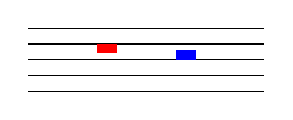
\begin{tikzpicture}
  \foreach \i in {-.4,-.2,0,.2,.4} \draw (0,\i) -- (3,\i);
  \fill[red] (.875,.08) rectangle ++ (.25,.12);
  \fill[blue] (1.875,0) rectangle ++ (.25,.12);
\end{tikzpicture}
\end{codeexample}
Other rests:
\begin{pictype}{tm-quarter-note-rest}{}
  Draw a quarter rest.
\end{pictype}
\begin{codeexample}[]
\begin{tikzpicture}
  \foreach \i in {-.4,-.2,0,.2,.4} \draw (0,\i) -- (2,\i);
  \pic[blue] at (1,0) {tm-quarter-note-rest};
\end{tikzpicture}
\end{codeexample}
For eighth rest and below, the pic name is |tm-|\meta{number}|-note-rest|, where 
\meta{number} is the number of `flags' in the rest notation. So |tm-1-note-rest| 
is the eighth rest, and so on. Currently \meta{number} must be either |1|,
|2|, |3| or |4|.
\begin{pictype}{tm-1-note-rest}{}
  Draw an eighth rest.
\end{pictype}
\begin{pictype}{tm-2-note-rest}{}
  Draw an sixteenth rest.
\end{pictype}
\begin{pictype}{tm-3-note-rest}{}
  Draw an thirty-second rest.
\end{pictype}
\begin{pictype}{tm-4-note-rest}{}
  Draw an sixty-fourth rest.
\end{pictype}
\begin{codeexample}[width=5.5cm]
\begin{tikzpicture}
  \foreach \i in {-.4,-.2,0,.2,.4} \draw (0,\i) -- (5,\i);
  \foreach \i in {1,2,3,4} \pic[blue] at (\i,0) {tm-\i-note-rest};
\end{tikzpicture}
\end{codeexample}

\subsubsection{Numbers}\label{sec:out:pic:numbers}
The pics draw musical numbers, taken from the music font \emph{Maestro}. Digit 
\meta{x} has a pic named |tm-number-|\meta{x}. By default, these pics are |4mm| 
high.
\foreach \i in {0,...,9} {%
\begin{pictype}{tm-number-\i}{}
  Draw number \i. \tikz\pic[scale=0.6]{tm-number-\i};
\end{pictype}%
}
Position in relative to the origin:
\begin{codeexample}[]
\begin{tikzpicture}
  \pic[scale=4] at (0,0) {tm-number-6};
  \draw[ultra thin,red] (0,1) -- (0,-1) (-1,0) -- (1,0);
\end{tikzpicture}
\end{codeexample}
\subsubsection{Other time signature notations}\label{sec:out:pic:time-signatures}
\begin{pictype}{tm-common-time}{}
  Draw common time notation. \tikz\pic[scale=0.6]{tm-common-time};
\end{pictype}
\begin{pictype}{tm-alla-breve-time}{}
  Draw alla breve time notation. \tikz\pic[scale=0.6]{tm-alla-breve-time};
\end{pictype}
\begin{codeexample}[]
\begin{tikzpicture}[scale=1.5,transform shape]
  \path (0,0) pic {tm-common-time} (1,0) pic {tm-alla-breve-time};
  \draw[ultra thin,red] (-.5,0) -- (1.5,0);
  \foreach \i in {0,1} \draw[ultra thin,red] (\i,.5) -- (\i,-.5);
\end{tikzpicture}
\end{codeexample}
\subsubsection{Accidentals}\label{sec:out:pic:accidentals}
\begin{pictype}{tm-sharp}{}
  Draw a sharp notation.
\end{pictype}
\begin{pictype}{tm-flat}{}
  Draw a flat notation.
\end{pictype}
\begin{pictype}{tm-natural}{}
  Draw a natural notation.
\end{pictype}
\begin{pictype}{tm-double-sharp}{}
  Draw a double sharp notation.
\end{pictype}
\begin{pictype}{tm-double-flat}{}
  Draw a double flat notation.
\end{pictype}
\begin{codeexample}[]
\begin{tikzpicture}[scale=1.5,transform shape]
  \foreach \i in {0,1,2,3,4} \draw[ultra thin,red] (\i,-.5) -- (\i,.5);
  \draw[ultra thin,red] (-.5,0) -- (4.5,0);
  \path (0,0) pic {tm-sharp} (1,0) pic {tm-flat} (2,0) pic {tm-natural}
    (3,0) pic {tm-double-sharp} (4,0) pic {tm-double-flat};
\end{tikzpicture}
\end{codeexample}
\subsubsection{Articulations}\label{sec:out:pic:articulations}
Only fermata notations are drawn using pics. Other articulations are all drawn 
using normal \tikzname\ commands. This is how those articulations are drawn 
internally:
\begin{codeexample}[]
\begin{tikzpicture}[scale=1.5,transform shape]
  \draw[line width=.1pt,red] (-.5,0) -- (4.5,0);
  \foreach \i in {0,1,2,3,4} \draw[line width=.1pt,red] (\i,.5) -- (\i,-.5);
  \fill[shift={(0,0)}] (0,0) circle (.4mm);%staccato
  \draw[shift={(1,0)}] (-.15,0) -- (.15,0);%tenuto
  \draw[shift={(2,0)}] (-.18,.075) -- (.18,0) -- (-.18,-.075);%accent above
  \fill[shift={(3,0)},rounded corners=.5pt]
    (0,.1) -- (-.04,-.075) to[out=-90,in=-90,looseness=2] (.04,-.075) -- cycle;%staccatissimo
  \draw[shift={(4,0)},fill]
    (-.1,-.1) -- (0,.1) -- (.1,-.1) -- (.033333,-.1) -- (-.033333,.0333333);%marcato
\end{tikzpicture}
\end{codeexample}
\begin{pictype}{tm-fermata-above}{}
  Draw a `fermata above' notation.
\end{pictype}
\begin{pictype}{tm-fermata-below}{}
  Draw a `fermata below' notation.
\end{pictype}
\begin{codeexample}[]
\begin{tikzpicture}
  \draw[line width=.1pt,red] (-.5,0) -- (1.5,0) (0,-.5) -- (0,.5) (1,-.5) -- (1,.5);
  \path (0,0) pic {tm-fermata-above} (1,0) pic {tm-fermata-below};
\end{tikzpicture}
\end{codeexample}
\subsubsection{Ornaments}\label{sec:out:pic:ornaments}
\begin{pictype}{tm-trill}{}
  Draw a trill.
\end{pictype}
\begin{pictype}{tm-turn}{}
  Draw a turn.
\end{pictype}
\begin{pictype}{tm-mordent}{}
  Draw a mordent.
\end{pictype}
\begin{codeexample}[width=5cm]
\begin{tikzpicture}[scale=1.5,transform shape]
  \draw[line width=.1pt,red] (-.5,0) -- (2.5,0);
  \foreach \i in {0,1,2} \draw[line width=.1pt,red] (\i,.5) -- (\i,-.5);
  \path (0,0) pic {tm-trill} (1,0) pic {tm-turn} (2,0) pic {tm-mordent};
\end{tikzpicture}
\end{codeexample}
That |tm-mordent| is the `upper' mordent. To have the `lower' version, this is 
how the package is drawing internally:
\begin{codeexample}[]
\begin{tikzpicture}[scale=2,transform shape]
  \draw[line width=.1pt,red] (-.5,0) -- (.5,0) (0,-.5) -- (0,.5);
  \path (0,0) pic {tm-mordent};
  \draw[line width=1pt] (0,-.15) -- (0,.15);
\end{tikzpicture}
\end{codeexample}
\subsubsection{Breath marks}\label{sec:out:pic:breath}
\begin{pictype}{tm-breath-mark}{}
  Draw a breath mark.
\end{pictype}
\begin{codeexample}[]
\begin{tikzpicture}[scale=2,transform shape]
  \draw[ultra thin,red] (-.5,0) -- (.5,0) (0,-.5) -- (0,.5);
  \pic at (0,0) {tm-breath-mark};
\end{tikzpicture}
\end{codeexample}
The caesura is not drawn using a pic. This is how it is drawn:
\begin{codeexample}[]

\begin{tikzpicture}[scale=2,transform shape]
  \foreach \i in {-.4,-.2,0,.2,.4} \draw (-.5,\i) -- (.5,\i);
  \fill[purple]
    (-.3,.2) -- (-.2,.2) -- (.1,.6) -- (0,.6) -- cycle
    (-.1,.2) -- (0,.2) -- (.3,.6) -- (.2,.6) -- cycle;
\end{tikzpicture}
\end{codeexample}
\subsubsection{Lines-related notations}\label{sec:out:pic:line}
Currently the following pics are defined:
\begin{pictype}{tm-8va}{}
  Draw a 8va notation.
\end{pictype}
\begin{pictype}{tm-8vb}{}
  Draw a 8vb notation.
\end{pictype}
\begin{pictype}{tm-15ma}{}
  Draw a 15ma notation.
\end{pictype}
\begin{pictype}{tm-15mb}{}
  Draw a 15mb notation.
\end{pictype}
\begin{codeexample}[width=4.5cm]
\foreach \i in {8va,8vb,15ma,15mb} {\tikz\pic{tm-\i};\quad}
\end{codeexample}
\begin{pictype}{tm-ped}{}
  Draw the stylised \emph{ped} used in pedal lines.
\end{pictype}
\begin{pictype}{tm-ped-star}{}
  Draw the star used in pedal lines.
\end{pictype}
\begin{codeexample}[]
\begin{tikzpicture}
  \draw (0,0) pic {tm-ped} -- (3,0) pic {tm-ped-star};
\end{tikzpicture}
\end{codeexample}
\subsubsection{Dynamics}\label{sec:out:pic:dynamics}
\foreach \i in {mf,f,ff,fff,mp,p,pp,ppp,fp} {%
\begin{pictype}{tm-dynamics-\i}{}
  Draw dynamics notation \texttt{\i}.
\end{pictype}%
}
\begin{codeexample}[]
\foreach \i in {mf,f,ff,fff,mp,p,pp,ppp,fp} {\tikz\pic{tm-dynamics-\i};\quad}
\end{codeexample}

\printindex
\end{document}